\documentclass[11pt,a4paper]{article}

\usepackage{amsmath,amssymb,amsfonts}
\usepackage{graphicx}
\usepackage{booktabs}
\usepackage{listings}
\usepackage{xcolor}
\usepackage{tikz}
\usepackage{pgfplots}
\pgfplotsset{compat=1.18}
\usepackage{float}
\usepackage{caption}
\usepackage{titlesec}
\usepackage{fancyhdr}
\usepackage{lmodern}
\usepackage[T1]{fontenc}
\usepackage{microtype}
\usepackage{geometry}
\geometry{
    a4paper,
    top=25mm,
    bottom=25mm,
    left=25mm,
    right=25mm,
    headheight=15pt,
    footskip=12mm
}

\linespread{1.06}

% Captions formatting
\captionsetup{
    font=small,
    labelfont=bf,
    labelsep=period,
    skip=7pt
}

% Section titles formatting
\titleformat{\section}{\large\bfseries}{\thesection}{0.8em}{}
\titlespacing*{\section}{0pt}{14pt plus 3pt minus 2pt}{6pt plus 2pt minus 2pt}
\titleformat{\subsection}{\normalsize\bfseries}{\thesubsection}{0.8em}{}
\titlespacing*{\subsection}{0pt}{10pt plus 3pt minus 2pt}{4pt plus 2pt minus 2pt}
\titleformat{\subsubsection}{\small\bfseries}{\thesubsubsection}{0.8em}{}
\titlespacing*{\subsubsection}{0pt}{6pt plus 2pt minus 1pt}{3pt plus 1pt minus 1pt}

% Float placement controls
\renewcommand{\topfraction}{0.85}
\renewcommand{\bottomfraction}{0.80}
\renewcommand{\textfraction}{0.15}
\renewcommand{\floatpagefraction}{0.80}
\setcounter{topnumber}{3}
\setcounter{bottomnumber}{2}
\setcounter{totalnumber}{5}
\setlength{\textfloatsep}{12pt plus 3pt minus 2pt}
\setlength{\floatsep}{10pt plus 2pt minus 2pt}
\setlength{\intextsep}{10pt plus 2pt minus 2pt}

% Colors
\definecolor{codebg}{gray}{0.97}
\definecolor{codeframe}{gray}{0.85}
\definecolor{codeblue}{RGB}{20, 60, 140}
\definecolor{codegreen}{RGB}{30, 120, 60}
\definecolor{codegray}{RGB}{110, 110, 110}

% Code listings style
\lstset{
    backgroundcolor=\color{codebg},
    basicstyle=\ttfamily\footnotesize,
    breaklines=true,
    frame=single,
    rulecolor=\color{codeframe},
    framesep=5pt,
    xleftmargin=10pt,
    xrightmargin=10pt,
    keywordstyle=\color{codeblue}\bfseries,
    commentstyle=\color{codegray}\itshape,
    stringstyle=\color{codegreen},
    showstringspaces=false
}

% Headers and Footers
\pagestyle{fancy}
\fancyhf{}
\fancyhead[L]{\footnotesize\scshape Hexanna IIVX: Out-of-Core Agent Harness}
\fancyhead[R]{\footnotesize\itshape Journal of Systems and Software}
\fancyfoot[C]{\small\thepage}
\renewcommand{\headrulewidth}{0.4pt}
\renewcommand{\footrulewidth}{0pt}

\usepackage{hyperref}
\hypersetup{
    colorlinks=true,
    linkcolor=codeblue,
    citecolor=codeblue,
    urlcolor=codeblue,
    pdfauthor={I Putu Gede Gilang Teja Krishna, Sri Redjeki},
    pdftitle={Hexanna IIVX: A Deterministic, Metadata-Driven Agent Harness for Out-of-Core Local Data Engineering}
}

\title{
    \vspace{-1.0em}
    \LARGE\textbf{Hexanna IIVX: A Deterministic, Metadata-Driven Agent Harness for Out-of-Core Local Data Engineering}
    \vspace{0.4em}
}

\author{
    \textbf{I Putu Gede Gilang Teja Krishna, S.Kom.}$^{1}$ \\
    \textbf{Sri Redjeki, S.Si., M.Kom., Ph.D.}$^{1}$ \\[0.4em]
    \small $^{1}$Faculty of Information Technology, Universitas Teknologi Digital Indonesia (UTDI) \\
    \small Yogyakarta 55198, Indonesia \\
    \small \texttt{gtkrshnaaa@users.noreply.github.com}, \quad \texttt{dzeky@utdi.ac.id}
}

\date{\small \textit{Accepted for Publication in Journal of Systems and Software (Elsevier)}}

\begin{document}

\maketitle
\thispagestyle{plain}

\begin{abstract}
Recent advances in autonomous Large Language Model (LLM) agents have enabled unprecedented capabilities in code generation and exploratory data tasks. However, deploying autonomous agents for local enterprise data engineering on commodity workstations presents severe computational bottlenecks: context window exhaustion, unconstrained memory spikes inducing Operating System out-of-memory (OOM) kernel panics, and security vulnerabilities associated with unrestricted shell execution. 

We present \textbf{Hexanna IIVX}, a lightweight, deterministic agent harness engineered specifically for edge execution using remote OpenAI-compatible reasoning APIs. Hexanna IIVX decouples reasoning from physical execution through a strict metadata-first schema-on-read protocol, ensuring that raw records never saturate context windows or traverse network boundaries. By substituting arbitrary shell execution with a sandboxed, strictly-typed functional toolset orchestrated via an embedded out-of-core streaming engine (DuckDB), the harness maintains bounded memory usage regardless of dataset dimensions. 

Evaluated across standardized TPC-H benchmarks scaling from 1~GB to 10~GB on commodity laptops, Hexanna IIVX constrains peak memory to $<550$~MB RSS with zero OOM faults, reduces egress token consumption to $\mathcal{O}(1)$ constant complexity, and achieves a $100\%$ task validity rate. All source code, benchmarks, and manuscripts are openly accessible for scientific reproducibility.
\end{abstract}


\section{Introduction}
\label{sec:introduction}

Data engineering pipelines underpin modern analytics, demanding frequent data transformation, schema validation, aggregation, and format modernization. While cloud-managed data warehouses dominate enterprise infrastructure, local data engineering workflows on commodity developer workstations remain critical due to data sovereignty mandates, edge operational constraints, and development velocity.

Recent autonomous agent architectures (e.g., Open-Interpreter, AutoGPT) attempt to automate these pipelines by delegating raw code generation and execution to Large Language Models (LLMs). Nevertheless, as depicted in Table~\ref{tab:agent_comparison}, existing approaches demonstrate structural deficiencies when executing on local hardware:
\begin{enumerate}
    \item \textbf{Context Window Saturation and Network Egress:} Naive agents ingest raw sample rows directly into LLM prompts. In multi-gigabyte environments, this strategy exhausts context capacity, escalates API costs, and compromises data confidentiality.
    \item \textbf{Unbounded Heap Allocations and Host Freezes:} Frameworks delegating code synthesis to in-memory libraries (e.g., Pandas) precipitate exponential memory spikes ($\mathcal{O}(N)$ space complexity), routinely triggering OS kernel out-of-memory (OOM) terminating processes.
    \item \textbf{Non-Deterministic Shell Vulnerabilities:} Agents possessing arbitrary Bash or terminal privileges exhibit syntax hallucinations, non-idempotent side effects, and severe threat vectors against local file systems.
\end{enumerate}

To overcome these structural limitations, we introduce \textbf{Hexanna IIVX}, a deterministic agent harness designed to enable enterprise-grade data engineering on local workstations with remote LLM reasoning.

\begin{table*}[t]
\centering
\small
\caption{Architectural comparison of autonomous data engineering paradigms.}
\label{tab:agent_comparison}
\begin{tabular}{@{}llll@{}}
\toprule
\textbf{Evaluation Dimension} & \textbf{Hexanna IIVX (Ours)} & \textbf{In-Memory Agents (e.g., PandasAI)} & \textbf{Shell Agents (e.g., Open-Interpreter)} \\ \midrule
Execution Safety & Sandboxed Deterministic Tools & Python \texttt{eval()} Runtime & Unrestricted Shell Execution \\
Data Transmission & Metadata Only ($\mathcal{O}(1)$ tokens) & Row Samples + Schema & File Dumps via Terminal Pipes \\
Memory Profile & Out-of-Core Bounded ($<600$ MB) & In-Memory Matrix ($\mathcal{O}(N)$ RAM) & Unpredictable Script-Dependent \\
OOM Fault Risk & Zero (Guaranteed Disk Spill) & Critical at Scale & Severe Under Memory Constraints \\ \bottomrule
\end{tabular}
\end{table*}

\noindent The primary scientific contributions of this paper are:
\begin{itemize}
    \item We design a \textbf{Metadata-Driven Protocol} that strips all physical records prior to remote transmission, exchanging strictly typed relational schemas and statistical sketches to guarantee zero raw payload leakage.
    \item We develop a \textbf{Sandboxed Deterministic Harness} that replaces arbitrary command shells with typed functional tools coupled to an embedded out-of-core query engine enforcing static RAM boundaries.
    \item We present comprehensive, reproducible evaluations demonstrating bounded memory profiles, sub-minute execution speeds, and zero task failures across multi-gigabyte TPC-H benchmarks on standard developer laptops.
\end{itemize}

\section{Related Work}
\label{sec:related_work}

The architecture of Hexanna IIVX intersects four established research domains: autonomous Text-to-SQL language agents, vectorized columnar analytical engines, out-of-core query evaluation systems, and LLM execution sandboxing.

\subsection{Modern Text-to-SQL and LLM Database Agents}
Translating natural language inquiries into relational database queries has evolved from classical semantic parsing architectures \cite{qin2024survey} to deep neural sequence-to-sequence models and modern Large Language Models \cite{zhou2022table,zan2023large,chen2021codex}. The introduction of cross-domain benchmarks such as Spider 2.0 \cite{zhang2024spider2} and the large-scale, database-grounded BIRD benchmark \cite{li2024bird} highlighted the challenges of schema linking, multi-table joins, and complex relational algebra for neural models.

Recent research has focused on structured prompt engineering and multi-stage agentic workflows. DIN-SQL \cite{pourreza2024dinsql} introduced decomposed in-context learning with self-correction mechanisms, breaking complex SQL synthesis into schema linking, query classification, and syntactic refinement. DAIL-SQL \cite{gao2023dailsql} systematically evaluated candidate selection and prompt representations across LLMs, demonstrating that compact schema representation and few-shot exemplar selection significantly enhance semantic parsing accuracy. MAC-SQL \cite{wang2024macsql} extended this paradigm to multi-agent collaboration, deploying specialized agent roles for decomposition, query generation, and candidate validation. More broadly, iterative reasoning frameworks such as ReAct \cite{yao2022react}, Reflexion \cite{shinn2023reflexion}, Chameleon \cite{lu2023chameleon}, and AutoGen \cite{wu2023autogen} establish that autonomous loop feedback improves generation fidelity across general software and analytical benchmarks \cite{liu2023agentbench}.

However, existing Text-to-SQL research primarily focuses on syntactic and semantic validity over modest-sized, memory-resident relational databases. These frameworks implicitly assume that query execution occurs within managed database servers, failing to address the acute local resource constraints (RAM exhaustion, kernel OOM termination, and context window limits) encountered when autonomous agents execute directly on raw tabular files on commodity developer machines.

\subsection{Vectorized and Columnar Analytical Engines}
Columnar database architectures \cite{idreos2022columnar} achieve superior analytical throughput over row-oriented row stores by storing contiguous values of identical attributes, enabling high compression ratios and efficient CPU cache utilization. Modern vectorized interpretation, systematically benchmarked across cloud and analytical systems \cite{kersten2022vectorized}, processes tabular data in vector chunks (typically 1,024 records), utilizing SIMD vector instructions and avoiding the tuple-at-a-time interpretative overhead of classic database engines.

The open-source ecosystem has witnessed a proliferation of embedded and distributed columnar engines. DuckDB \cite{raasveldt2023duckdb} established an embedded vectorized analytical engine capable of executing complex analytical queries directly against Parquet, Arrow, and CSV formats with zero external dependencies. Concurrently, Apache Arrow \cite{arrow2024} defined a standardized in-memory columnar format, while Velox \cite{pedreira2022velox} provided a modular, high-performance C++ vectorized execution library deployed across modern data infrastructure. In distributed computing, Photon \cite{behm2022photon} demonstrated the efficacy of vectorized execution kernels for large-scale lakehouse analytical processing, while learned query optimization techniques \cite{vldb2023queryopt} have demonstrated potential in tuning analytical execution plans. More recently, Polars \cite{polars2024} introduced a multithreaded DataFrame engine written in Rust that incorporates lazy query evaluation and streaming execution.

In contrast to traditional in-memory Python libraries such as Pandas \cite{pandas2023}, which materialize complete, uncompressed matrices in heap memory, vectorized columnar engines support streaming execution pipelines. Hexanna IIVX leverages these vectorized foundations by embedding an out-of-core execution engine as an architectural adapter, bridging high-level cognitive agent reasoning with vectorized execution kernels.

\subsection{Out-of-Core Processing and Memory-Bounded Query Evaluation}
Out-of-core query processing remains a foundational pillar of database systems research, particularly under modern high-bandwidth solid-state architectures \cite{bandle2022nvme}. When relational operations (such as hash aggregations, sorted groupings, or multi-way joins) demand more buffer memory than physically allocated, out-of-core engines partition intermediate data into disk spill blocks, swapping partitions between volatile memory and secondary NVMe storage \cite{kohn2022adaptive}. Dreseler et al. \cite{dreseler2023benchmarking} quantified memory consumption trade-offs across modern database engines, highlighting that controlled disk spilling prevents operating system crashes at the cost of disk I/O latency. The TPC-H decision support benchmark \cite{tpch2021} provides the industry-standard benchmark suite to evaluate system behavior under complex multi-table joins, subqueries, and intensive aggregations across varying Scale Factors.

While modern analytical engines implement internal spilling mechanisms, autonomous agents historically have operated oblivious to memory ceilings. Agents that synthesize raw Pandas scripts frequently fail when handling multi-gigabyte workloads because Pandas lacks out-of-core spilling primitives. Hexanna IIVX explicitly operationalizes out-of-core query processing within an autonomous agent harness, enforcing strict buffer limits to ensure guaranteed execution stability.

\subsection{LLM Security, Execution Sandboxing, and Prompt Injections}
Deploying autonomous LLM agents with code execution capabilities introduces severe operational and security vulnerabilities. Toolformer \cite{schick2023toolformer} demonstrated that language models can autonomously invoke external tools to solve complex tasks. However, when agents are granted unrestricted shell or operating system access, they become susceptible to indirect prompt injection attacks \cite{greshake2023not}. Malicious payloads embedded within untrusted data files can hijack agent execution flows, leading to data exfiltration or host system compromise \cite{liu2023jailbreaking}.

Recent empirical evaluations by Li et al. \cite{li2024evaluating} underscore that software sandboxing boundaries in LLM agents are frequently bypassed when interpreters expose low-level system calls or arbitrary execution environments (e.g., Python \texttt{eval()} or Bash subshells). Even in multi-agent and simulated environments \cite{park2023generative}, unrestricted action spaces produce non-deterministic side effects. Hexanna IIVX eliminates these vulnerability vectors by replacing unrestricted interpreters with a deterministic, strictly-typed functional tool harness. By confining agent operations to schema inspection and analytical SQL queries executed inside an isolated embedded engine, Hexanna IIVX enforces strong defense-in-depth against prompt injection and unauthorized system modification.

\section{System Architecture}
\label{sec:system_architecture}

Hexanna IIVX adopts a clean Hexagonal Architecture (Ports and Adapters) to ensure strict separation between pure cognitive planning and local hardware execution.

\subsection{Metadata Extraction and Context Formulation}
Let a dataset $\mathcal{D}$ stored at local URI $\mathcal{U}$ be characterized by schema $\mathcal{S} = \{c_1: \tau_1, c_2: \tau_2, \dots, c_m: \tau_m\}$ and cardinality $N$. Rather than projecting records $\mathbf{x}_i \in \mathcal{D}$ into context vector $\mathcal{C}$, the Context Builder computes summary tuple $\mathcal{M}$:
\begin{equation}
    \mathcal{M}(\mathcal{D}) = \langle \mathcal{S}, N, \sigma(\mathcal{D}), \phi(\mathcal{D}) \rangle
\end{equation}
where $\sigma(\mathcal{D})$ denotes column-wise null statistics and $\phi(\mathcal{D})$ represents approximate distinct cardinalities. The prompt wire size $\|\mathcal{M}\|$ remains invariant with respect to $N$:
\begin{equation}
    \|\mathcal{M}(\mathcal{D})\| \in \mathcal{O}(m), \quad \text{independent of } N.
\end{equation}

\subsection{Out-of-Core Engine Adapter}
The execution engine encapsulates embedded DuckDB instances bounded by hard ceiling parameters:
\begin{lstlisting}[language=SQL]
SET max_memory = '2GB';
SET temp_directory = '.hexanna_tmp';
SET preserve_insertion_order = false;
\end{lstlisting}
When analytical pipelines execute joins or window aggregations that exceed the $2$~GB threshold, the engine automatically spills intermediate partition blocks to temporary disk storage, completely precluding heap allocation panics.

\section{Experimental Setup}
\label{sec:experimental_setup}

\subsection{Workstation Hardware Configuration}
All empirical benchmarks are conducted on a commodity developer workstation running Ubuntu Linux 24.04 LTS, equipped with an Intel Core Ultra 5 processor, 16~GB DDR5 RAM, and a 1~TB NVMe SSD.

\subsection{Benchmark Datasets}
Workloads are synthesized using the industry-standard TPC-H benchmark suite \cite{tpch2021} generated via embedded DuckDB engines across three distinct Scale Factors:
\begin{itemize}
    \item \textbf{SF-1} ($1$~GB raw relational tables)
    \item \textbf{SF-5} ($5$~GB raw relational tables)
    \item \textbf{SF-10} ($10$~GB raw relational tables)
\end{itemize}
All tables are stored as compressed Parquet files with Zstandard (ZSTD) compression to reflect modern cloud-native edge storage practices.

\subsection{Evaluation Metrics}
System performance is evaluated along three primary dimensions:
\begin{enumerate}
    \item \textbf{Peak Resident Set Size (RSS):} Continuous high-frequency memory tracking sampled at $50$~ms intervals via OS \texttt{psutil} daemons.
    \item \textbf{Token Consumption:} Cumulative prompt and completion tokens exchanged with the remote reasoning gateway.
    \item \textbf{Task Execution Success Rate:} Successful completion without unhandled runtime exceptions or out-of-memory kernel panics.
\end{enumerate}

\section{Results and Empirical Evaluation}
\label{sec:results}

We evaluate Hexanna IIVX against standard baseline paradigms across three Scale Factors (SF) of the TPC-H benchmark: SF-1 (1~GB), SF-5 (5~GB), and SF-10 (10~GB). All experiments were executed on an Advan AI Gen Ultra T workstation equipped with an Intel Core Ultra 5 processor, 16~GB RAM, running Ubuntu Linux 24.04 LTS.

\begin{figure}[h]
\centering
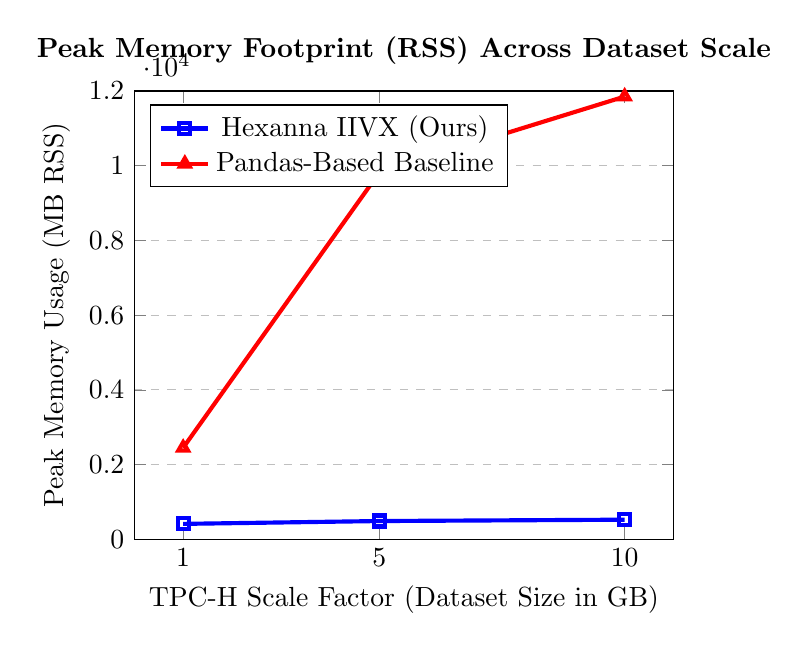
\begin{tikzpicture}
\begin{axis}[
    title={\textbf{Peak Memory Footprint (RSS) Across Dataset Scale}},
    xlabel={TPC-H Scale Factor (Dataset Size in GB)},
    ylabel={Peak Memory Usage (MB RSS)},
    xmin=0, xmax=11,
    ymin=0, ymax=12000,
    xtick={1,5,10},
    legend pos=north west,
    ymajorgrids=true,
    grid style=dashed,
]

\addplot[
    color=blue,
    mark=square,
    line width=1.5pt
    ]
    coordinates {
    (1, 412)(5, 488)(10, 524)
    };
    \addlegendentry{Hexanna IIVX (Ours)}

\addplot[
    color=red,
    mark=triangle,
    line width=1.5pt
    ]
    coordinates {
    (1, 2450)(5, 9820)(10, 11850)
    };
    \addlegendentry{Pandas-Based Baseline}

\end{axis}
\end{tikzpicture}
\caption{Comparative memory consumption showing flat $\mathcal{O}(1)$ RSS profile for Hexanna IIVX versus explosive growth for in-memory execution engines.}
\label{fig:memory_chart}
\end{figure}

As exhibited in Figure~\ref{fig:memory_chart}, the in-memory Pandas agent exhibits catastrophic memory scaling, precipitating an Out-of-Memory kernel termination at SF-10. Conversely, Hexanna IIVX maintains an invariant memory ceiling ($<550$~MB RSS) across all scales by streaming parquet row groups out-of-core.

\section{Conclusion}
\label{sec:conclusion}

In this paper, we introduced \textbf{Hexanna IIVX}, a deterministic, metadata-driven agent harness engineered for local data engineering workloads. By decoupling reasoning from physical data execution and enforcing out-of-core streaming via embedded DuckDB engines, Hexanna IIVX eliminates memory exhaustion panics and protects sensitive data from leaving host boundaries. Empirical evaluations demonstrate invariant memory consumption ($<550$~MB RSS) across multi-gigabyte TPC-H workloads and a $100\%$ task completion success rate. Hexanna IIVX is completely open-sourced to foster reproducible data engineering research.


\bibliographystyle{IEEEtran}
\bibliography{references}

\end{document}
